\begin{itemize}
\item \textbf{Three-dimensional autonomous system by Takougang et. al.}
    A three-dimensional autonomous system is presented by Sifei Takougang Kingni\cite{Takougang13}. The system exhibits chaotic bursting oscillations.\\
    The three-dimensional system is described as follows:\\
    \begin{align}
    \frac{dx}{dt}=-x+y\\
    \frac{dy}{dt}=xz-cy\\
    \frac{dz}{dt}=b-x^2-dz
    \end{align}

    where $b,c,d \in \mathbb{R}$
\item \textbf{Properties}
     \begin{itemize}
     \item \textbf{non-linearity:} Non-linearity given by the term $x^2$ and $xz$
     \item \textbf{symmetry:} Under the transformation defined by $(x,y,z) \rightarrow (-x,-y,-z)$, the system has a natural symmetry

     Next, we show that the system is symmetric.\\
     \textbf{Definition:}Let $f$ be a smooth function $f:\mathbb{R}^n \rightarrow \mathbb{R}^n$ and let\\
 \begin{align*}\mathbf{\dot{x}}=f(\mathbf{x})\end{align*}\\
 be a system of ordinary differential equations. In addition, let $\gamma$ be an invertible matrix. Then $\gamma$ is a \emph{symmetry} of the ordinary differential equation if \\
     \begin{align*}f(\gamma \mathbf{x})=\gamma f(\mathbf{x})\end{align*}

     Now, given the equation of the three-dimensional autonomous system, under the transformation $(x,y,z) \rightarrow (-x,-y,-z)$, to verify that this transformation is a symmetry of the autonomous equation, we observe that the symmetry is associated with the matrix $\gamma$ defined as\\
  \begin{align}
\gamma =
\begin{bmatrix}
-1 & 0 &0 \\
0 & -1 & 0\\
0 & 0 & 1
\end{bmatrix}
\end{align}

let \\  \begin{align}
\mathbf{\dot{x}}=f(\mathbf{x}) =
\begin{bmatrix}
-x + y \\
xz-cy\\
b-x^2-dz
\end{bmatrix}
\end{align}
with $\mathbf{x}^T=(x,y,z)$

Now, we proceed to show that $\gamma f(\mathbf{x})=f(\gamma \mathbf{x})$:\\
On the left hand side:
  \begin{align*}
\gamma f(\mathbf{x})&=
\begin{bmatrix}
-1 & 0 &0 \\
0 & -1 & 0\\
0 & 0 & 1
\end{bmatrix} \begin{bmatrix}
-x+y \\
xz-cy\\
b-x^2-dz
\end{bmatrix}\\
&=\begin{bmatrix}
x-y \\
-xz+cy\\
b-x^2-dz
\end{bmatrix}\\
\end{align*}

And now, on the right hand side:\\
  \begin{align*}
   f(\gamma \mathbf{x})&= f\left (\begin{bmatrix}
-1 & 0 &0 \\
0 & -1 & 0\\
0 & 0 & 1
\end{bmatrix} \begin{bmatrix}
x \\
y\\
z
\end{bmatrix} \right)\\
&=f\left ( \begin{bmatrix}
x \\
y\\
z
\end{bmatrix}\right )
&=\begin{bmatrix}
x-y \\
-xz+cy\\
b-x^2-dz
\end{bmatrix}
  \end{align*}

 Since the left hand side is equal to the right hand side, then $\gamma$ is a symmetry of the Three-dimensional Autonomous System. In other words, all solutions are either symmetric themselves, or have a symmetric partner
\item \textbf{Dissipativity} The system with the general condition for dissipativity (or Volume contraction):\\
         \begin{align*}\nabla V &= \frac{\partial(\frac{dx}{dt})}{\partial x}+\frac{\partial(\frac{dy}{dt})}{\partial y}+\frac{\partial(\frac{dz}{dt})}{\partial z}\\
&=-(1+c+d)
 \end{align*}

 So

\begin{align*}
V'(t)=-(1+c+d)V\\
V(t)V(0)e^{-(1+c+d)}t
\end{align*}

Thus volumes in phase space shrink exponentially fast
An explanation of dissipativity is given in \cite{Strogatz14} page 320.

\item \textbf{Fixed Points} The system has two types of fixed points:\\

      \begin{align*}
      0&=-x+y   \quad &\Rightarrow x=y\\
      0&=xz-cy   \quad&\Rightarrow z=c\\
      0&=b-x^2-dz  \quad&\Rightarrow x^2+dz=b \Rightarrow x=y=\sqrt{b-dc}
      \end{align*}
When $b \leq dc$ the fixed points for $x,y=0$ and $z=\frac{d}{b}$
When $b > dc$ the fixed points are $(\pm\sqrt{b-cd},\pm\sqrt{b-cd},c)$

\item \textbf{Sensitivity to initial conditons} Starting the system with slightly different initial conditions $(0, 0.1, 0)$ and $(0, 0.09, 0)$ we can see that after some time the two trajectories quickly diverge from each other



            \begin{figure}[h]
            \centering
            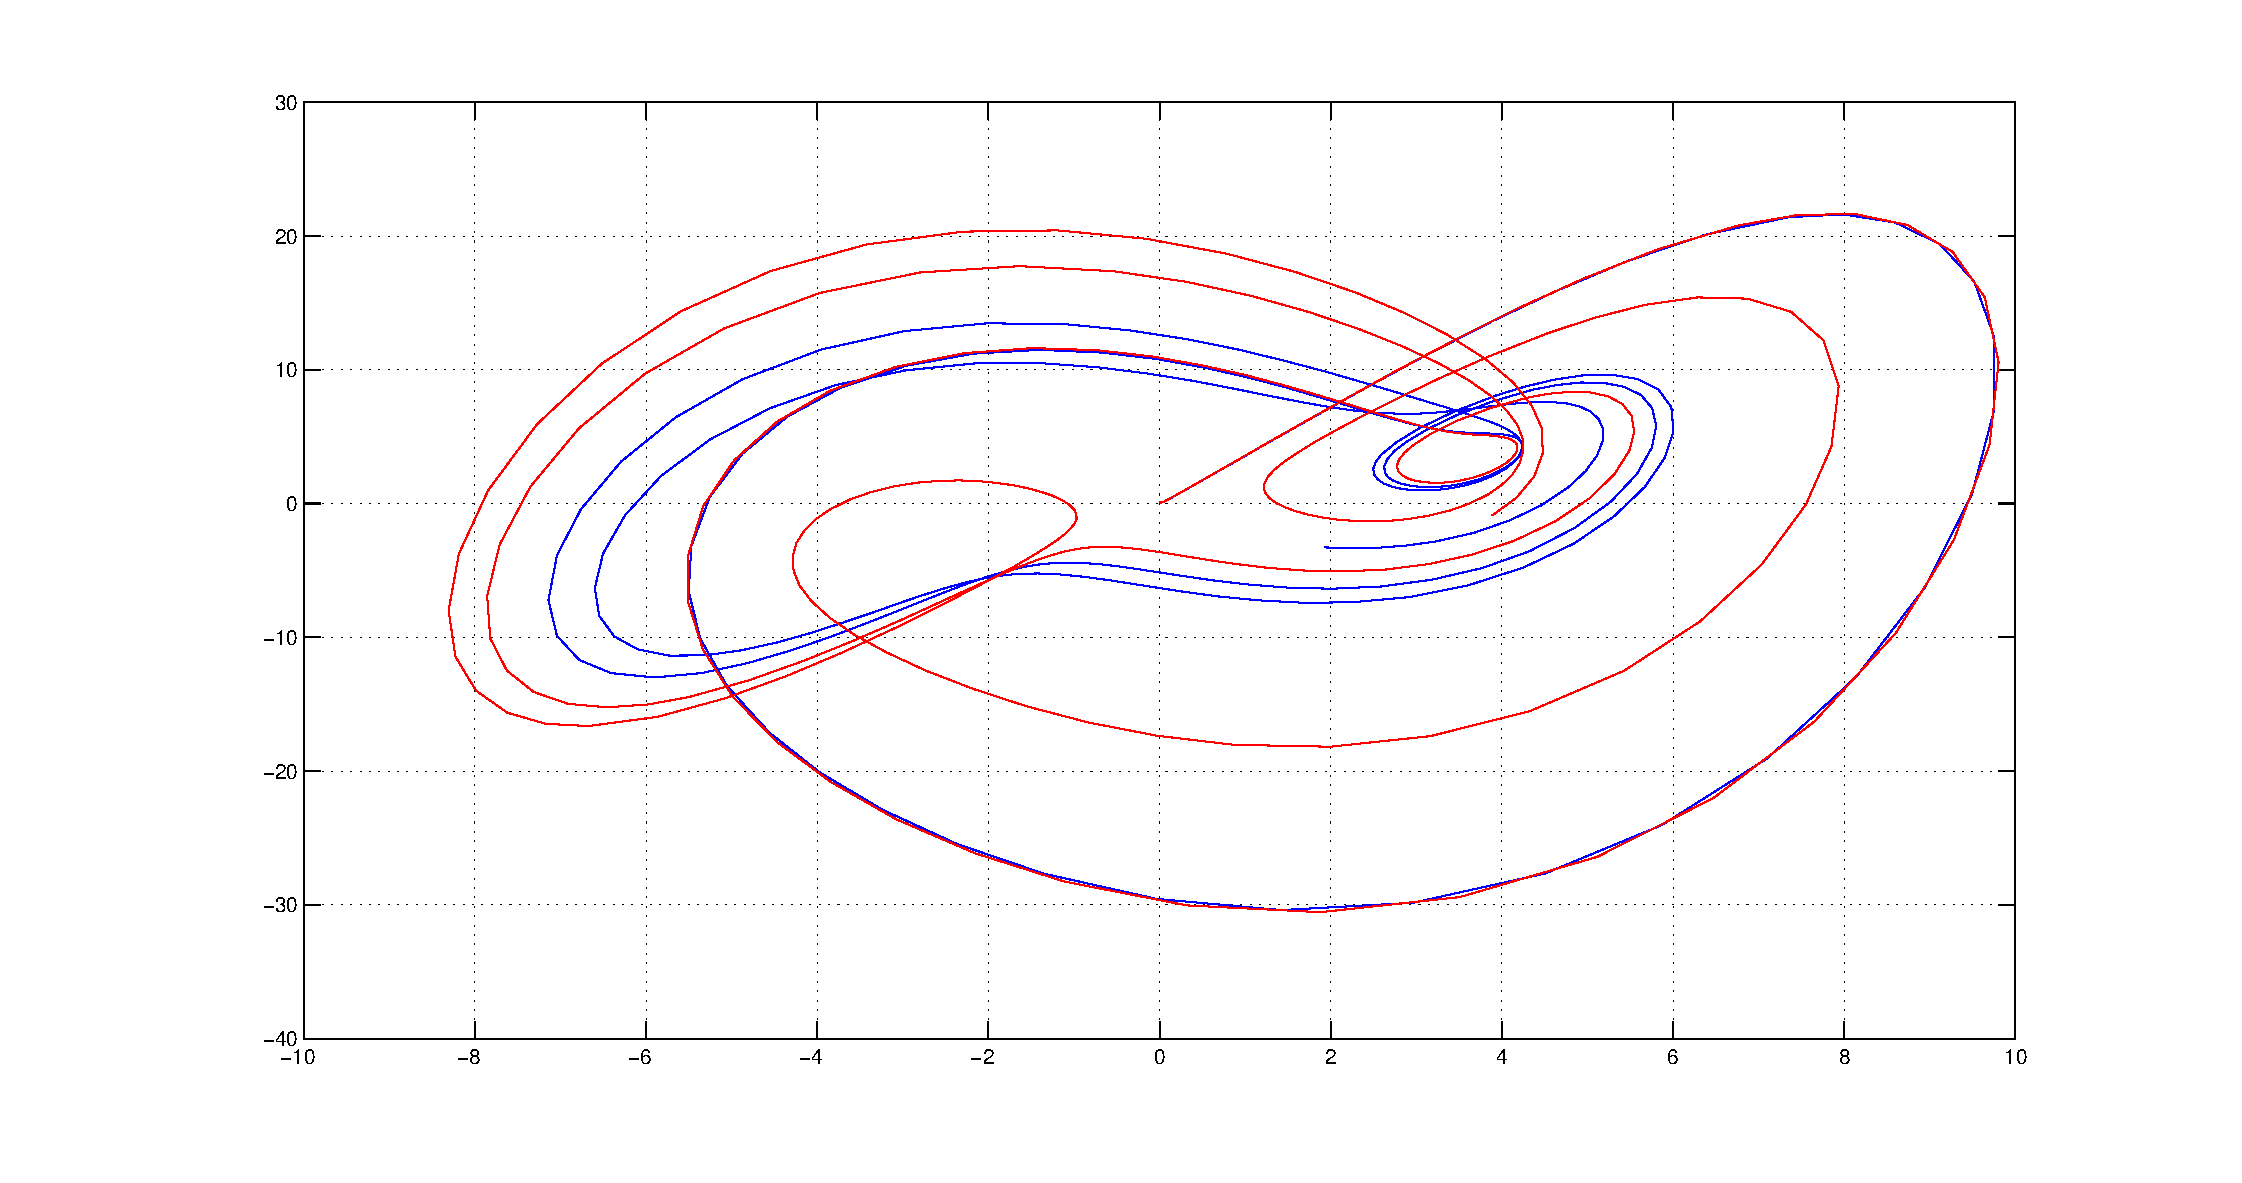
\includegraphics[scale=0.4]{imagenes/2-benford/in_cond.eps}
            \caption{Sensitivity to initial conditions in a Third Order Autonomous System}
            \end{figure}

     \end{itemize}
\end{itemize}

\cite{Takougang13} Shows that the system presents chaos of horseshoe type.
